% %% Mustervorlage für eine Studienarbeit am LS VS/BS



% % % !TeX spellcheck = en_US
% \documentclass[ twoside,openright,titlepage,numbers=noenddot,%headinclude,%1headlines,% letterpaper a4paper
% %\documentclass[ titlepage,numbers=noenddot,%headinclude,%1headlines,% letterpaper a4paper
%                 footinclude=true,abstractoff, % <--- obsolete, remove (todo)
%                 %cleardoublepage=empty,
%                 cleardoublepage=plain,
%                 BCOR=3mm,paper=b5,fontsize=11pt,11pt,%a4paper,%
%                 british,open=right%
%                 ]{scrreprt}
% \usepackage[utf8]{inputenc}

% %
% % (Re-)Add support for the deprecated font commands
% %
% \makeatletter
% \DeclareOldFontCommand{\rm}{\normalfont\rmfamily}{\mathrm}
% \DeclareOldFontCommand{\sf}{\normalfont\sffamily}{\mathsf}
% \DeclareOldFontCommand{\tt}{\normalfont\ttfamily}{\mathtt}
% \DeclareOldFontCommand{\bf}{\normalfont\bfseries}{\mathbf}
% \DeclareOldFontCommand{\it}{\normalfont\itshape}{\mathit}
% \DeclareOldFontCommand{\sl}{\normalfont\slshape}{\@nomath\sl}
% \DeclareOldFontCommand{\sc}{\normalfont\scshape}{\@nomath\sc}
% \makeatother

% %    * New enumeration (small caps): \begin{aenumerate} \end{aenumerate}
% %    * For margin notes: \marginpar or \graffito{}
% %    * See classicthesis-preamble.sty for useful commands

% %********************************************************************
% % Note: Make all your adjustments in here
% %*******************************************************
% \usepackage[dvipsnames]{xcolor}

% \usepackage[T1]{fontenc}
% \usepackage[estonian,finnish,swedish,english]{babel}


%\cefoot{\pagemark}
%\cofoot{\pagemark}
%put the page number in the center of the page


% \usepackage{multirow}
% \usepackage{flafter}
% \usepackage{multirow}
% \usepackage{siunitx}
% \usepackage{caption}
% \usepackage{subcaption}
% \usepackage{acronym}
% \usepackage{listings}
% \usepackage{color}
% \usepackage{pdflscape}
% \usepackage{longtable}
% \usepackage{dcolumn}
% \usepackage{relsize}
% \usepackage{marvosym}
% \usepackage{needspace}
% \usepackage{pdfpages}
% %\newcolumntype{d}[1]{D{.}{\ldot}{#1} }
% \usepackage[numbers]{natbib}
% %\usepackage[style=authoryear,backend=biber]{biblatex}
% \usepackage[gen]{eurosym}

% \sisetup{per=fraction}
% \DeclareSIUnit\COe{\ce{CO2}e}
% \DeclareSIUnit\cubicmetre{\metre\cubed}
% \DeclareSIUnit\Euro{\euro{}}
% \DeclareSIUnit\GBP{£}
% \DeclareSIUnit\Hertz{Hz}
% \DeclareSIUnit\day{d}
% \DeclareSIUnit\byte{B}

\documentclass[12pt, a4paper,English]{scrreprt}
\usepackage[a4paper, width=150mm, top=25mm, bottom=25mm, bindingoffset=1mm]{geometry}


\usepackage{ae}
\usepackage{aecompl}
\usepackage[T1]{fontenc}
% \usepackage[latin1]{inputenc}
\usepackage[utf8]{inputenc} 
\usepackage{amsmath}
\usepackage{graphicx}
\graphicspath{{images/}}
\usepackage{amssymb}
\usepackage [chapter]{tocbibind}
\usepackage{latexsym}
\usepackage{multicol}
\usepackage[english]{babel}
\usepackage[utf8]{inputenc}
\usepackage{my-preamble}
\usepackage{svg}
\usepackage[numbers]{natbib}
\usepackage{setspace}
% \usepackage[style=authoryear, sorting=ynt]{biblatex}
% \addbibresource{library.bib}
% \usepackage{classicthesis-preamble}
% \usepackage{classicthesis}
\usepackage[hyphen]{url} %break long urls in bibliography
\usepackage{acronym}
\usepackage{tocloft}
\usepackage{algpseudocode}
\usepackage[chapter]{algorithm}

\setkomafont{chapter}{\normalfont\Large\lifamily\bfseries}
\setkomafont{section}{\normalfont\normalsize\lifamily\bfseries}

\makeatletter
\renewcommand\chapterlinesformat[3]{%
  \@hangfrom{#2}{\MakeUppercase{#3}}%
}
\makeatother
\renewcommand\chapterlineswithprefixformat[3]{%
  \MakeUppercase{#2#3}%
}




%*******************************************************
% Font selection
%*******************************************************
\usepackage{libertine}

%*******************************************************
% Fine-tuning for the text area
%*******************************************************
\linespread{1.2} % a bit more for Libertine

\usepackage[automark]{scrlayer-scrpage}
\automark{chapter}
\clearpairofpagestyles
\cfoot[\pagemark]{\pagemark}
% \lehead{\headmark}
\rohead{\headmark}
\pagestyle{scrheadings}


% \usepackage{fancyhdr}
% \pagestyle{fancy}
% \fancyhead{}
% \fancyhead[RO,LE]{Thesis Title}
% \fancyfoot{}
% \renewcommand{\headrulewidth}{0.4pt}
% \renewcommand{\footrulewidth}{0.4pt}
% \pagestyle{scrheadings}
% \ofoot[]{}
% \ifoot[]{}
% \cfoot[\pagemark]{\pagemark}

%hier könnt ihr weitere Pakete einfügen, falls ihr diese benötigt
\typearea[current]{current}

%%es folgen Definitionen für das Titelblatt
%%An geeigneter Stelle ist der Text anzupassen

\begin{document}



\begin{titlepage}
    \begin{center}
        
        \LARGE  

        
\includegraphics[width=0.7\textwidth]{images/euroaquae-logo.png} 

        \hfill

        \vfill

        
        \textbf{\myTitle}

        \vfill
        
        \large{\myNameCaps}
        
        \vfill
        
        {\Large \myTime}
         
    \end{center} 
\end{titlepage}



\newpage\null\thispagestyle{empty}\newpage
% \thispagestyle{empty}


% \titlehead{\vspace{0cm}
\includegraphics[width=0.5\textwidth]{btu-logo.jpg}
% \hspace{1cm}
\includegraphics[width=0.3\textwidth]{fluidit-logo.pdf}
% }

% % Logos next to each other
% % \subject{\vspace{1cm}
\includegraphics[width=0.5\textwidth]{btu-logo.pdf}
% % \hspace{0.5cm}
\includegraphics[width=0.3\textwidth]{fluidit-logo.pdf}}

% % \subject{\vspace{1cm}
\includegraphics[width=0.5\textwidth]{btu-logo.jpg}
% % \hspace{0.5cm}
\includegraphics[width=0.3\textwidth]{fluidit-logo.pdf}}



% \title{\vspace{3cm}Continuous simulation of urban sanitary sewer network}


% \author{Pedro Paulo Almeida Silva \\ EuroAquae+ Student}

% \date{\textit{\\April 2019}}



% \publishers{

% 1. Academic Supervisor: Dr. Frank Molkenthin  \\ 2. Institutional Supervisor: Dr. Markus Sunela

% }






\thispagestyle{empty}

\hfill
%\begin{addmargin}[-1cm]{1cm}  

\begin{center}

%\myFaculty\\
%\myDepartment\\
{\large BRANDENBURG UNIVERSITY OF TECHNOLOGY COTTBUS-SENFTENBERG} \\
{Erasmus Mundus Joint Master Programme}\\

\bigskip
\end{center}


\medskip

{\small
\noindent{\textbf{This dissertation was accepted as the final thesis report of the degree of \myDegree in Hydroinformatics and Water Management.}}

\vspace{0.5cm}
\noindent{
\begin{tabular}{ll}
{\textbf{Academic Supervisor}}:& \mySupervisorII \vspace{-.1cm}\\
\vspace{-.1cm}&\mySupervisorLabII \\
\vspace{-.1cm}&\mySupervisorLocationII\\
\\
{\textbf{Institutional Supervisor}}:&\mySupervisor \vspace{-.1cm}\\
\vspace{-.1cm}&\mySupervisorLab ,\\
\vspace{-.1cm}&\mySupervisorLocation\\
\\

\end{tabular}}


\noindent{\textbf{Thesis Presentation:} \myPresentationTime}

\medskip
\vspace{0.5cm}

\noindent{\textbf{Funding:} \\
{Euroaquae is a joint Master Programme funded by Erasmus+. This dissertation also received support from Fluidit Oy company where the student performed a professional practice with the title of Master Thesis Worker.}


\noindent

\includegraphics[width=0.5\textwidth]{images/fundederasmus.png}
\hspace{3cm}

\includegraphics[width=0.3\textwidth]{images/fluidit-logo.pdf}


\vspace{0.25cm}


\noindent{\textbf{Declaration:} \\
\textit{I hereby declare that this work was written independently without any unauthorized assistance or sources not given credit within the work. All words, phrases, passages, and data taken from other sources have been properly cited. No parts of this work in the same form or a similar form have ever been previously handed in to fulfill an examination.}}

\begin{flushright}
    \begin{tabular}{r}
        \\ \hline
        \myName \\
    \end{tabular}
\end{flushright}
\vspace{1cm}

%\noindent{Colophon: 
%This thesis was typeset with \LaTeXe\ using Andr\'e Miede's
%\emph{classicthesis} style with modifications by David Schryer and
%Ardo Illaste to conform with Tallinn University of Technology style guidelines. The %main font is
%Libertine (Times compatible). Biolinum is used for sans-serif text.}
%\vfill
%\medskip

% \noindent{Copyright: \myName, \myYear\\}
% ISSN 1406-4766\\
% ISBN 978-9949-83-165-4 (publication)\\
% ISBN 978-9949-83-166-1 (PDF)}}

%\end{addmargin}

\noindent

\includegraphics[width=0.3\textwidth]{images/btu-logo.jpg}
\hspace{0.3cm}

\includegraphics[width=0.2\textwidth]{images/NU-logo.png}
\hspace{0.3cm}

\includegraphics[width=0.15\textwidth]{images/WUT-Symbol.jpg}
\hspace{0.3cm}

\includegraphics[width=0.2\textwidth]{images/PNS-logo.png}
\hspace{0.3cm}

\includegraphics[width=0.08\textwidth]{images/UPC-logo.png}



\pagenumbering{roman}

% \setlength\cftparskip{-0.5pt}
% \setlength\cftbeforechapskip{0pt}
% \tableofcontents
% \newpage
% \listoffigures
% \newpage
% \listoftables
% \clearpage



\setlength\cftparskip{-0.5pt}
\setlength\cftbeforechapskip{0pt}
\tableofcontents
\newpage


\setlength\cftparskip{-0.5pt}
\setlength\cftbeforechapskip{0pt}
\listoftables
\newpage


\setlength\cftparskip{-0.5pt}
\setlength\cftbeforechapskip{0pt}
\listoffigures
\newpage

\phantomsection\addcontentsline{toc}{chapter}{\tocEntry{Abstract}}
\chapter*{Abstract}
[To Do]

will be completed when final results are obtained.

\phantomsection\addcontentsline{toc}{chapter}{\tocEntry{Dedication}}
\chapter*{Dedication}

\phantomsection\addcontentsline{toc}{chapter}{\tocEntry{Acknowledgements}}
\chapter*{Acknowledgements}

\phantomsection\addcontentsline{toc}{chapter}{\tocEntry{Acronyms}}
\chapter*{Acronyms}
\begin{acronym}[AMALGAM]
  \addtolength{\itemsep}{-2mm}
\acro{BWF}{Base Wastewater Flow}
\acro{CSN}{Combined Sewer network}
\acro{CSO}{Combined Sewer Overflow}
\acro{DDS}{Dynamically Dimensioned Search}
\acro{DEM}{Digital Elevation Model}
\acro{DWF}{Dry-Weather Flow}
\acro{EPA}{U.S. Envinronmental Protection Agency}
\acro{FMI}{Finnish Meteorological Institute}
\acro{HD-DDS}{Hybrid Discrete Dynamically Dimensioned Search}
\acro{I/I}{Infiltration and Inflow}
\acro{NLS}{Finnish National Land Survey}
\acro{RDII}{Rainfall-derived Infiltration and Inflow Real}
\acro{SCADA}{Supervisory Control and Data Access}
\acro{SSN}{Sanitary Sewer network}
\acro{SSOAP}{Sanitary Sewer O Analysis and Planning}
\acro{SSO}{Sanitary Sewer Overflow}
\acro{SYKE}{Finnish Environment Institute}
\acro{SWMM}{Stormwater Management Model}
\acro{TMF}{Traffic Management Finland}
\acro{UH}{Unit Hydrograph}
\acro{WWF}{Wet-Weather Flow}
\acro{WWTP}{Wastewater Treatment Plant}
\acro{XML}{Extensible Markup Language}
\end{acronym}    


%=========================================
% Return page number style to Arabic
%=========================================
\newcounter{runningpage}
\setcounter{runningpage}{\value{page}}
\pagenumbering{arabic}
\setcounter{page}{\value{runningpage}}
%=========================================


\chapter{Introduction}
%Introduction
Modelling sanitary sewer network flows allow cities to understand and solve issues that impact its society, environment and economy. To model sanitary sewer network flows, it is first necessary to identify the behavior of the system. As described by \citet{Vallabhaneni2007} the flows in the network usually have two different behaviors that are classified as: 1. dry-weather flow (DWF); 2. wet-weather flow (WWF). To apply a continuous simulation and successfully forecast the flows in the sanitary sewer system, the model should be able to account for both DWF and WWF.

Typically, DWF pattern can be estimated by analyzing historical data from flow measurements available along the network or at the downstream end during dry periods \cite{Bennett1999}. Intuitively, usually more water is discharged into the sewer in day time than during the night. More complexity is added when trying to estimate WWF in the sanitary sewer network. Flow increases in the network due to inflow and infiltration often trigged by rainfall or snowmelt. This incremental quantity of flow which finds its way into the sanitary sewer network during a rainfall event is known by Rainfall Dependent Inflow and Infiltration (RDII).

The challenge on RDII estimations lies upon the different ways stormwater enters a sanitary or combined sewer \cite{Mosley2001}. Stormwater can inflow to the sanitary or combined sewer network directly through foundation and roof drains connections, leaky manhole covers, or stormwater drains.  Infiltration occurs due to defects in the network components such as: damaged pipes, joints, manholes, etc. \cite{Rossman2016}
Quantity of inflow and infiltration (I\&I) increases proportionally with intensity of the rainfall and snowmelt. Urban areas located in cold climate can have a significant inflow due to snowmelt and was, therefore, considered during this study. For that, the incremental flow caused by snowmelt will be referred here as Snowmelt Dependent Inflow and Infiltration (SDII). Event-based Inflow and Infiltration (EBII) will be used as a general term for both snowmelt and rainfall inflow and infiltration.


\begin{figure}[ht]
    \centering
	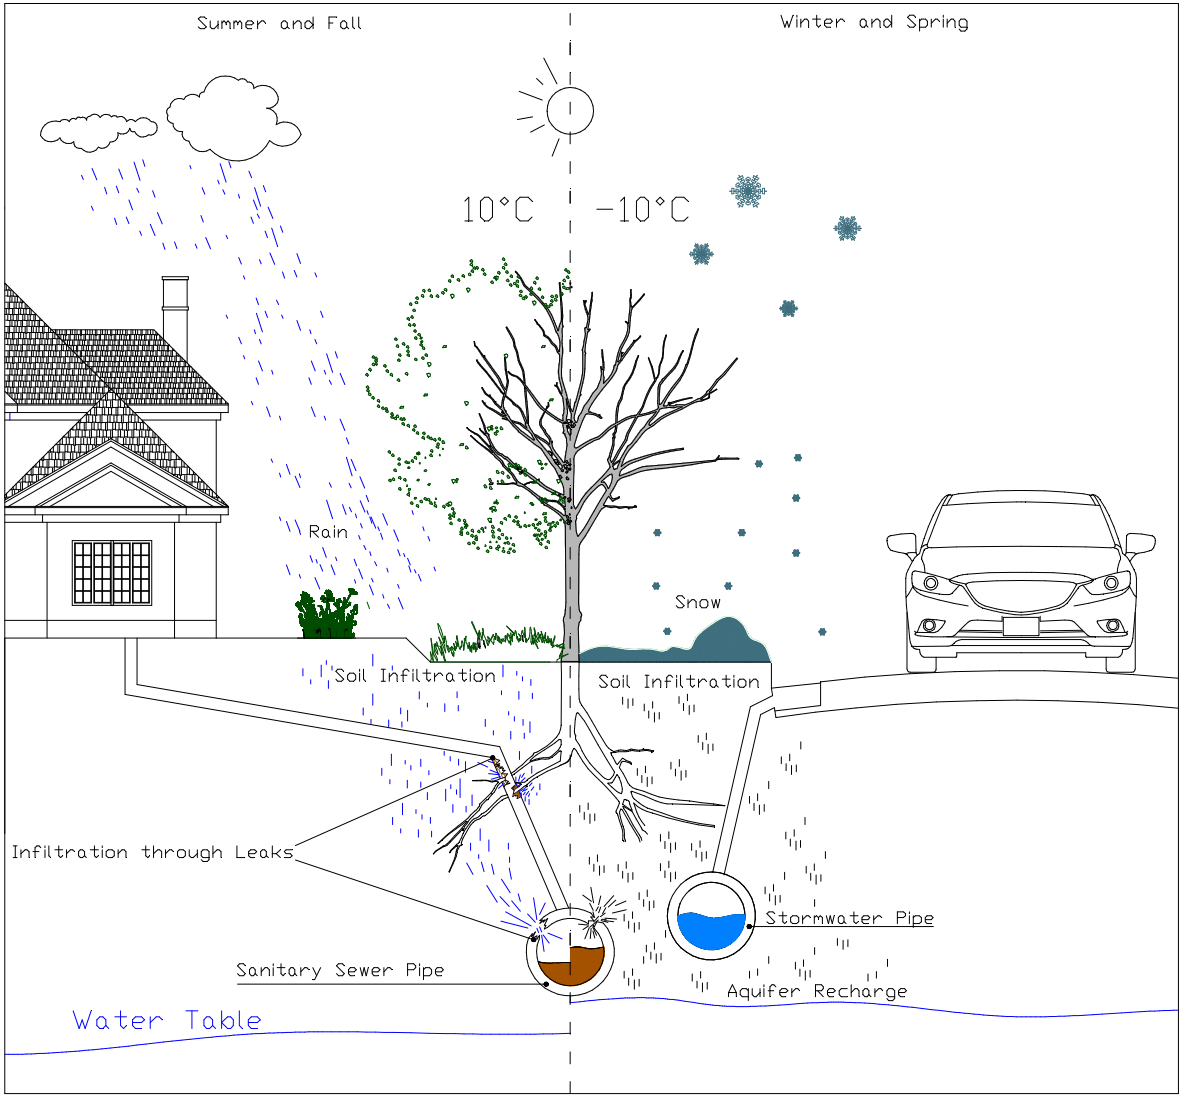
\includegraphics[scale=0.62]{figures/sanitary_sewer_leakage.png}
	\caption{Wet-weather Infiltration}
	\label{fig:wetinf}
\end{figure}


\section{Motivation}
Event-base inflow and infiltration (EBII) causes increase of the quantity of flow into sanitary sewer systems. This increase may cause sanitary sewer overflow (SSO) due to exceedance of the system capacity  \cite{Rossman2016}. In some cities, sanitary sewer is combined with stormwater sewer network. The capacity of this coupled systems may also be exceeded during an event causing combined sewer overflow (CSO) \cite{Vallabhaneni2007}. When the capacity is exceeded, untreated water rejected by the wastewater treatment plants (WWTPs) is released into surface waters \cite{DeRodaHusman2016} such rivers and streams. Upstream capacity-related issues may cause wastewater to find its way into basements or streets \cite{Roesner2009}. Untreated water released on the surface water bodies or urban area increases the risk of human contamination by infectious diseases. 
Although these are well known problems, they are still present in urban centers around the globe. Frequency of CSOs are seasonal dependent. The current prediction of more frequent intensive rainfall events also increases the frequency of CSO \cite{DeRodaHusman2016} and enlarge the damage caused by these overflows. Moreover, wastewater overflows can cause conflicts in the society when streams or rivers are used both as an option to dispose wastewater and recreational area as described by \citet{heikkinen2016}. To give cities, municipalities and water utilities the ability to predict SSOs and CSOs is one of the motivations of this study. However, other benefits are also aimed. A continuous simulation considering urban hydrology and hydraulics can also be used to improve the service and reduce operational costs for water utilities. 
EBII can increase the inflow of wastewater to WWTPs for weeks due to possible long response times \cite{Mosley2001}. Obviously, the operational cost of the plant will increase since more wastewater needs to be treated. A continuous simulation might be able to identify increases over time on the flow pattern in specific pipes or sub-divisions of the network. This would be an indicator for the water utility to carry further inspections and evaluate whether the infrastructure is damaged allowing infiltration. Furthermore, a digital model of the network gives to the water utilities the ability to analyze the impacts on the whole network caused by changes in the network such as: decommissioning of a water tower, changing pumping schedule, or analyzing impacts of a future new neighborhood. 





\chapter{Methodology}

To tackle the issues presented in the previous section, this study will investigate the main aspects behind the development of two hydraulic models with the aim to approximate the behavior of the sanitary sewer network flows continuously in a cold climate influenced by annual snowmelt periods. In the future, the model should be able to cope with existing monitoring infrastructure of \acf{SCADA} and weather forecast data as input to predict the future status of the network. Even though this study does not go as far as description of real implementation of an integrated operational and CSOs/SSOs early warning system, it focuses the development and data acquisition of the hydrological models in real-time operation. It is important to keep in mind the purpose of the model since it influenced decisions of methods to be used and data fetching routines. Thus, key aspects of this study involves:
\begin{itemize}
    \item fetching of real-time monitoring data;
    \item automatic calibration \& validation;
    \item State of network in different nodes;
    \item Transfer times among pumping stations;
    \item 24h forecast: possible overflows, capacities, etc.
\end{itemize}

There is an existent hydraulic model of the study site. Therefore, details about this model are briefly presented later in section \ref{hydraulicmodel}.
Focus is given here to the hydrological model and the methodology was divided in two parts named: 1. Offline Model and 2. Online Model. The first aimed to investigate the model's data necessities, the process of parameter estimation based on spatial data of the study site, and first simulation with previously estimated parameters. The Online Model uses not only historical meteorological events, but also weather forecast for comparing the two proposed hydraulic models results and a preliminary analysis of their performance for real-time applications. 

\section{Offline Model}
First step was the creation of hydrological model and coupling to hydraulic model using \acf{SWMM} developed by the \acf{EPA}. The model was built, calibrated and validated using historical data. The goal of the offline model part was to identify the best set of parameters and how to handle challenging parts such as: initial soil moisture content, soil frost, percentage of rainfall lost to stormwater sewer network, aquifer interations, etc. Figure \ref{fig:offlineflow} shows a simplified flowchart of the hydrological model development steps.


\begin{figure}[h]
    \centering
	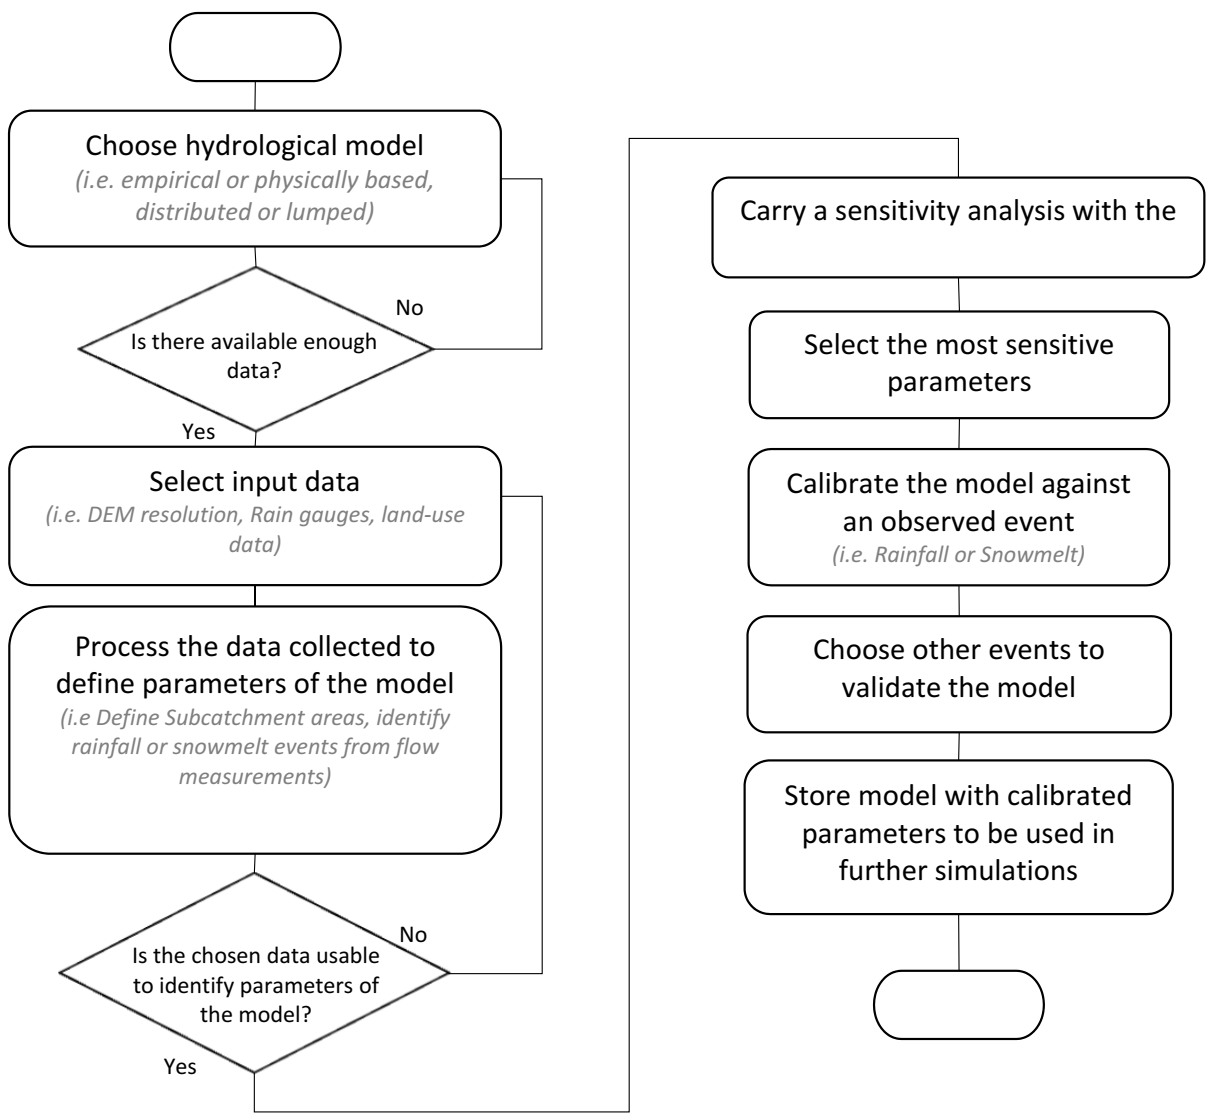
\includegraphics[height=12cm]{figures/Offline_Model_Creation_Flow_Chart.png}
	\caption{Hydrological Model Development Flowchart}
	\label{fig:offlineflow}
\end{figure}



\section{Online Model}

[To Do]

\textbf{This section will aim to answer the questions posed below} \\ \\

This section presents questions related to the continuous simulation process. The answers express initial ideas to explain how the continuous simulation will work and what are the main concerns. 
•	How long will the simulations run? This depends on many factors such as the type of hydrological, hydraulic model, calibration process, routine, hardware used to process the information. 

•	How often will the simulation run? Routine of simulation is constraint by data acquisition routine.  The routine of simulation can also vary during a storm event applying a shorter time of simulation. As an example, imagine if all necessary data to run a simulation is available every 15min and the model takes 30min to run a complete simulation, the iterations necessary for the optimization of parameters during the calibration process can be reduced as an attempt to decrease the time of simulation down to 15min. This could allow a better decision-making process during intense rainfall events, even if some accuracy is compromised.

•	What information is relevant before, during, and after a rainfall or snowmelt event?
Before the rainfall and/or snowmelt: When and where peak flows will happen in the sanitary sewer system. Where and when can CSOs or SSOs can happen. What would be the transfer times between points of the network? During rainfall and/or snowmelt: Status of the system with focus in short-time forecast (+1-2h): Where are the peak flows, CSOs, SSOs, happening and how will then be within 1-2h. Are all the measurement instruments safe and providing good enough data? Maybe a quick check of the input data will be necessary to identify whether the instrument is broken or not. If we cannot rely on the real-time data, what would be the strategy? Maybe use the last reliable data collected to forecast the behavior of the system. After rainfall and/or snowmelt:  Maybe the peak flows will still happen. How long will the flows in the system still be considered RDII and higher than average peak flows of DWF? 

•	Which parameters will be calibrated? According do Choi and Ball (2002) (Choi and Ball 2002) there are two types of parameters related to quantity part of runoff block in SWMM: 1. Measured Parameters; 2. Inferred Parameters. The first are parameters directly measured such length of channels/pipes, catchment land-use, or recorded rainfall depth. The second, parameters not directly measured, and coefficients used by empirical models that approximate complex physical processes. More about this is discussed in section 4.4. Inferred parameters approximate characteristics of the system (i.e. imperviousness) and processes (i.e. flow coefficients such as hydraulic conductivity or manning’s). Inferred parameters are the least known values since no measurements were carried. Therefore, they are the first candidates to be chosen when calibrating since the uncertainties tend to be higher than the measured parameters. A sensitivity analysis will be done during the offline modelling part to identify which of the inferred parameters have greater impact to the results. The inferred parameters with greater impacts will be then chosen for calibration. 

•	Why not all parameters will be calibrated? The number of parameters necessary to run SWMM and the range of possible values for each parameter can be a very large number. This increases the search space for the calibration algorithm where many iterations will be required to identify optimal set of parameters. This can rapidly increase the time of simulation limiting the model’s forecast capability.

•	How will the Automatic Calibration Process work? The automatic calibration will have a routine according to the necessity of the models. A calibration run might happen in scale of hours, days, weeks, months, etc. A new set of parameters will then be proposed and an evaluation to compare whether the new set of parameters is better than the previous one. The frequency of calibration and the possible values of the parameters must be further investigated since less frequent events might have very distinct behavior than more frequent events. It is also possible to define different set of parameters for different seasons and event’s magnitude. An approximated system diagram is shown in figure \ref{fig:diagram}.


\begin{figure}[h]
    \centering
	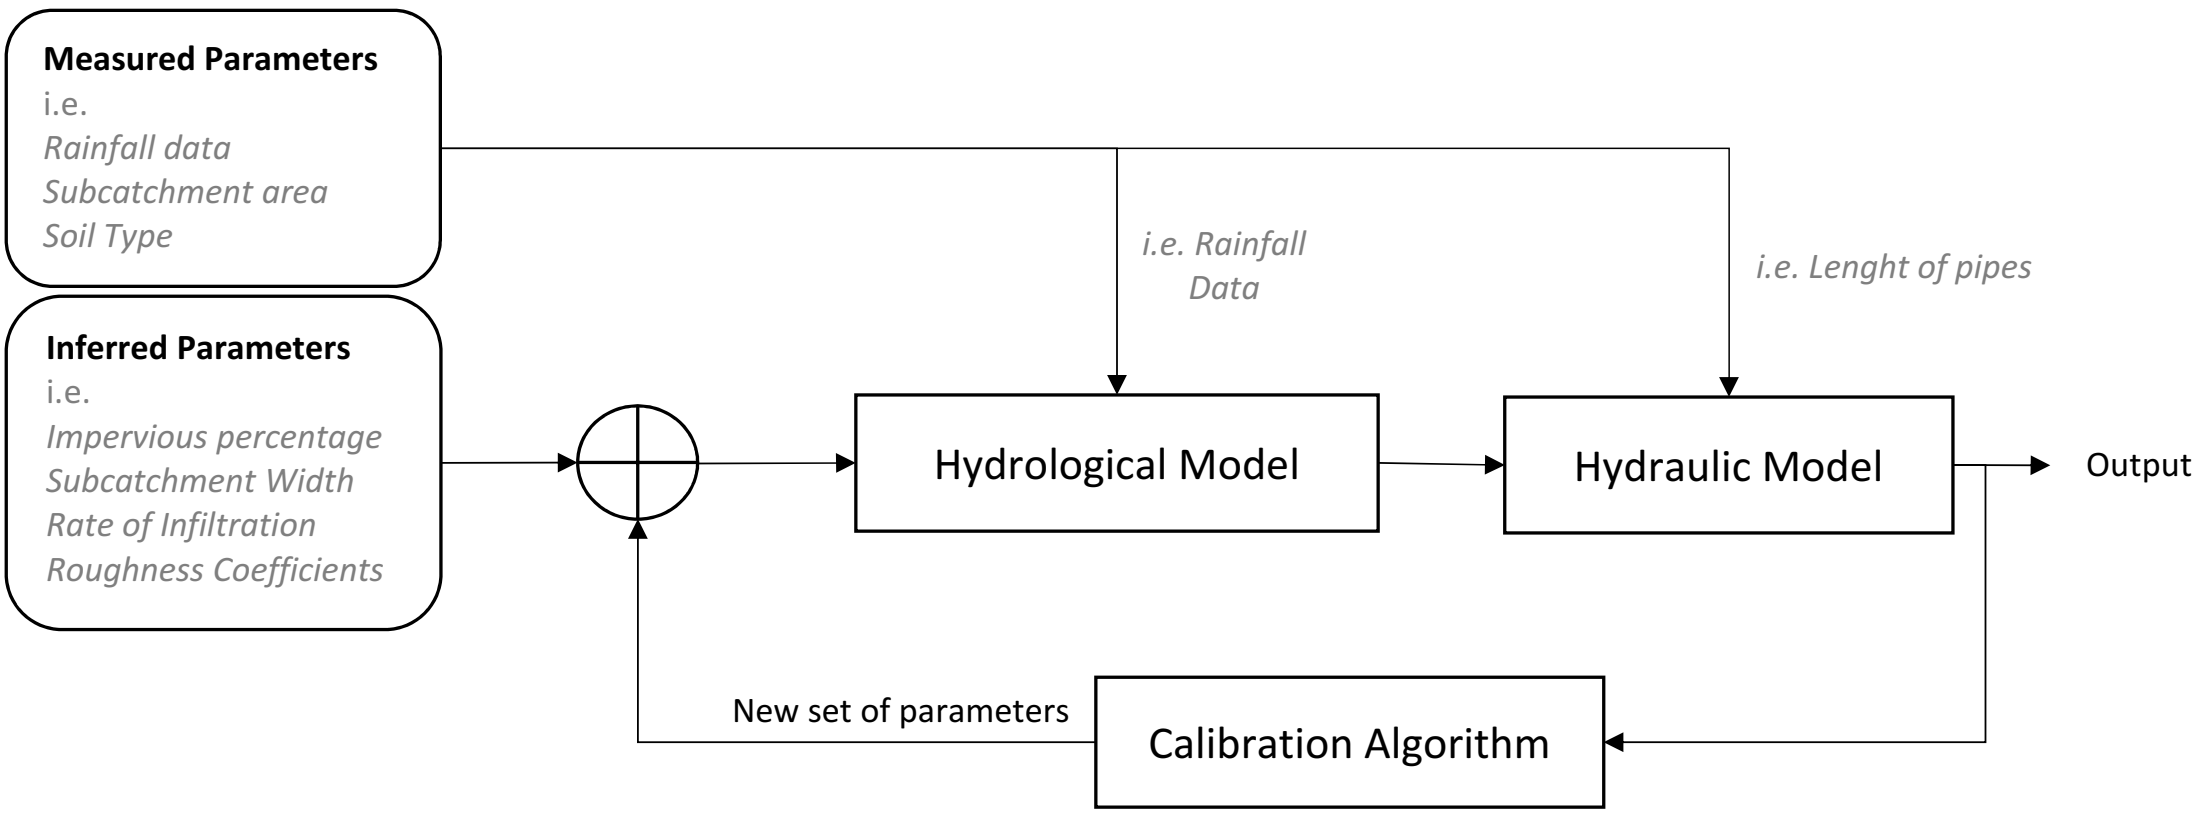
\includegraphics[scale=0.35]{figures/System_Diagram.png}
	\caption{System Diagram}
	\label{fig:diagram}
\end{figure}


\section{Parameter Optimization Algorithm}

\acf{DDS} is a stochastic single-solution based heuristic global search algorithm that was created for the automatic calibration process of watershed simulation models. It was developed to find good global solution for a set of parameters faster than previously available search algorithms. DDS was proposed by \citeauthor{tolson2007} \citeyearpar{tolson2007}  \cite{tolson2007}. 
DDS mimics the process of manual calibration. According to \citet{dent2004} a calibration algorithm workflow can be defined as: 
\begin{enumerate}
    \item Change parameters of the model;
    \item Run the model simulation;
    \item Measure error of simulated vs observed;
    \item Repeat previous steps and choose the most fit set of parameters.
\end{enumerate}
For hydrologic models with multiple subcatchments and parameters, the number of possible combinations of parameters are of several orders of magnitude. This complexity motivates the adoption of optimization algorithms for automatic calibration.   
For a given hydrologic model with only one catchment and three different parameters: area, slope, and roughness. Assuming that area is constant but the other two can assume each five other possible values. The possible combination of parameters to represent the catchment would be 165. Now let’s assume the catchments is divided in two subcatchments. In this case, the possible number of combinations would raise to 74613.
The name Dynamically Dimensioned is given due to the ability of the algorithm to scale the search based on user-specified maximum number of iterations. Global search approach is used for the first iterations. DDS switches to a local search approach by selecting and reducing the search space when the number of iterations nears the maximum allowed. The algorithm reduces the search space by strategic reduction of the number of parameters to be calibrated when it approximates to the end of the search. It also respects the constraints of each parameter given by the user. Therefore, it does not choose values for a parameter out of the specified range.
Other relevant aspects of Automatic Calibration and DDS for SWMM:


\begin{itemize}
    \item Automatic Calibration avoids modelers bias, accelerates the process of calibration, and handles multiple objectives such as peak flows, hydrograph shape, and total volume \cite{dent2004};
    \item DDS was created for computationally expensive calibrations \cite{arsenault2013}. Therefore, it is suitable for SWMM where a possible large number of parameters should be simultaneously optimized;
    \item DDS converges rapidly finding a good solution for a set of parameters and successfully avoid poor local solutions \cite{tolson2007};
    \item For distributed model such as used in SWMM, comparisons available in the literature have proven that DDS is one of the fastest to converge and the best finding good solutions. In other words, DDS does outperform other algorithms for complex models\cite{tolson2007,wallner2012,arsenault2013};
\end{itemize}

\begin{algorithm}
	\caption{Dynamically dimensioned search algorithm by \citet{tolson2007} and algorithm structure presentation by \citet{Sunela2017}}
	\label{alg:dds}
	\begin{algorithmic}
		\State $f_{best} \gets f(\bar{x}_0)$
		\State $\bar{x}_{best} = \bar{x}_0$
		\For {$i \gets 1,\,m$}
		\State \textit{Randomly select the decision variables that will be perturbed.}
		\State $p \gets 1 - \frac{\ln{i}}{\ln{m}}$
		\State $N \gets \emptyset$
		\For {$d \gets 1,\,n$} 	
		\State $X \sim U([0, 1])$
		\State \textbf{if} $X \leq p$ \textbf{then}	$N \gets N \cup \{d\}$
		\EndFor
		\If {$N = \emptyset$}
		\Comment{Ensure variable change}
		\State $X \sim U([1, n])$
		\State $N = \{ X \}$
		\EndIf
		\State \textit{Construct new solution by perturbing the current best}
		\State $\bar{x} \gets \bar{x}_{best}$
		\For {$\forall j \in N$}
		\State $x_j \gets x^{best}_j + r \cdot (x^{max}_j - x^{min}_j) \cdot N([0, 1])$		
		\If{$x_j < x^{min}_j$}
		\State $x_j \gets x^{min}_j + (x^{min}_j - x_j)$
		\State \textbf{if} $x_j > x^{max}_j$ \textbf{then} $x_j \gets x^{min}_j$
		\ElsIf{$x_j > x^{max}_j$}
		\State $x_j \gets x^{max}_j - (x_j - x^{max}_j)$
		\State \textbf{if} $x_j < x^{min}_j$ \textbf{then} $x_j \gets x^{max}_j$
		\EndIf
		\EndFor
		
		\State \textit{Evaluate the objective function value for the new solution}
		\State $f \gets f(\bar{x})$
		\If{$f \leq f_{best}$}
		\State $f_{best} = f$
		\State $\bar{x}_{best} = \bar{x}$
		\EndIf
		\EndFor
	\end{algorithmic}	
\end{algorithm}



 



\chapter{Hydrological Model}




Flow in the sanitary sewer network can be classified as Dry-Weather Flow (DWF) and Wet-Weather Flow (WWF). DWF can be further divided in two components: 1. Base Waste Flow (BWF): inflow of waste water coming from households, commercial and industrial sites; and 2. Groundwater Infiltration (GWI): Water from aquifers that infiltrates into the network thought defects such as pipe cracks and leaky joints(Vallabhaneni and Burgess 2007). 
The choice of the hydrological model in this study aims the representation of RDII, which is the incremental flow into the sanitary sewer system caused by precipitation (rainfall or snowmelt). Figure 3 shows the typical characteristics of different components of sanitary sewer flow. RDII needs to be first separated from DWF when processing raw data coming from flow meters. More about the methods to separate the components are discussed on section 4.2.


\begin{figure}[ht]
    \centering
	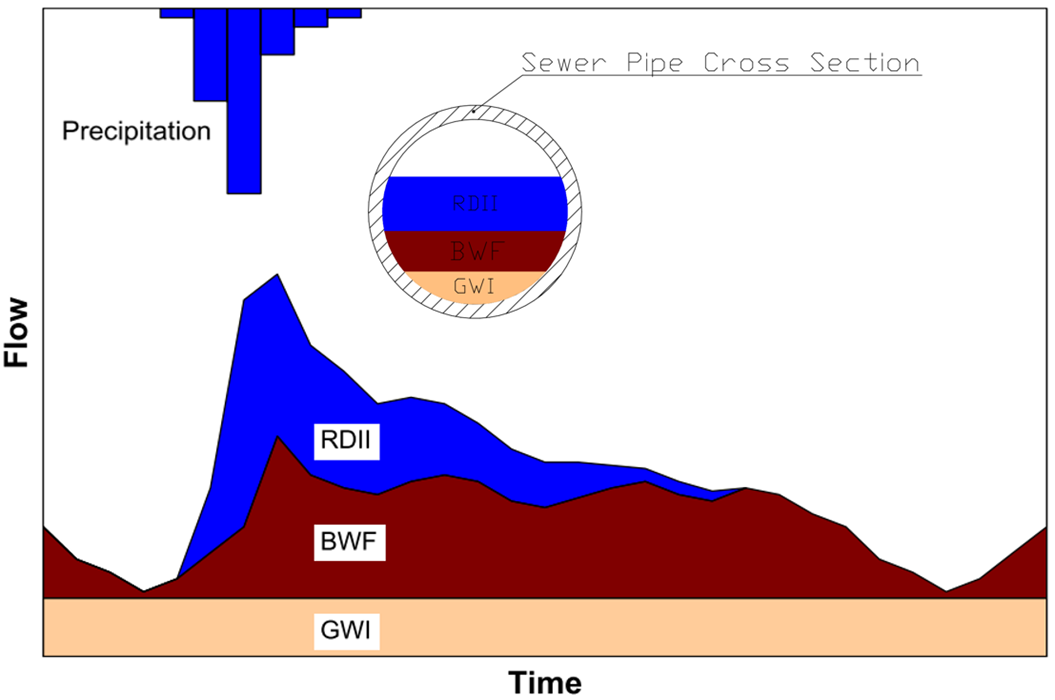
\includegraphics[scale=0.6]{figures/RDII_flows.png}
	\caption{Wet-weather flow components. Modified from \cite{Vallabhaneni2007}}
	\label{fig:flowcomponents}
\end{figure}


\begin{figure}[ht]
    \centering
	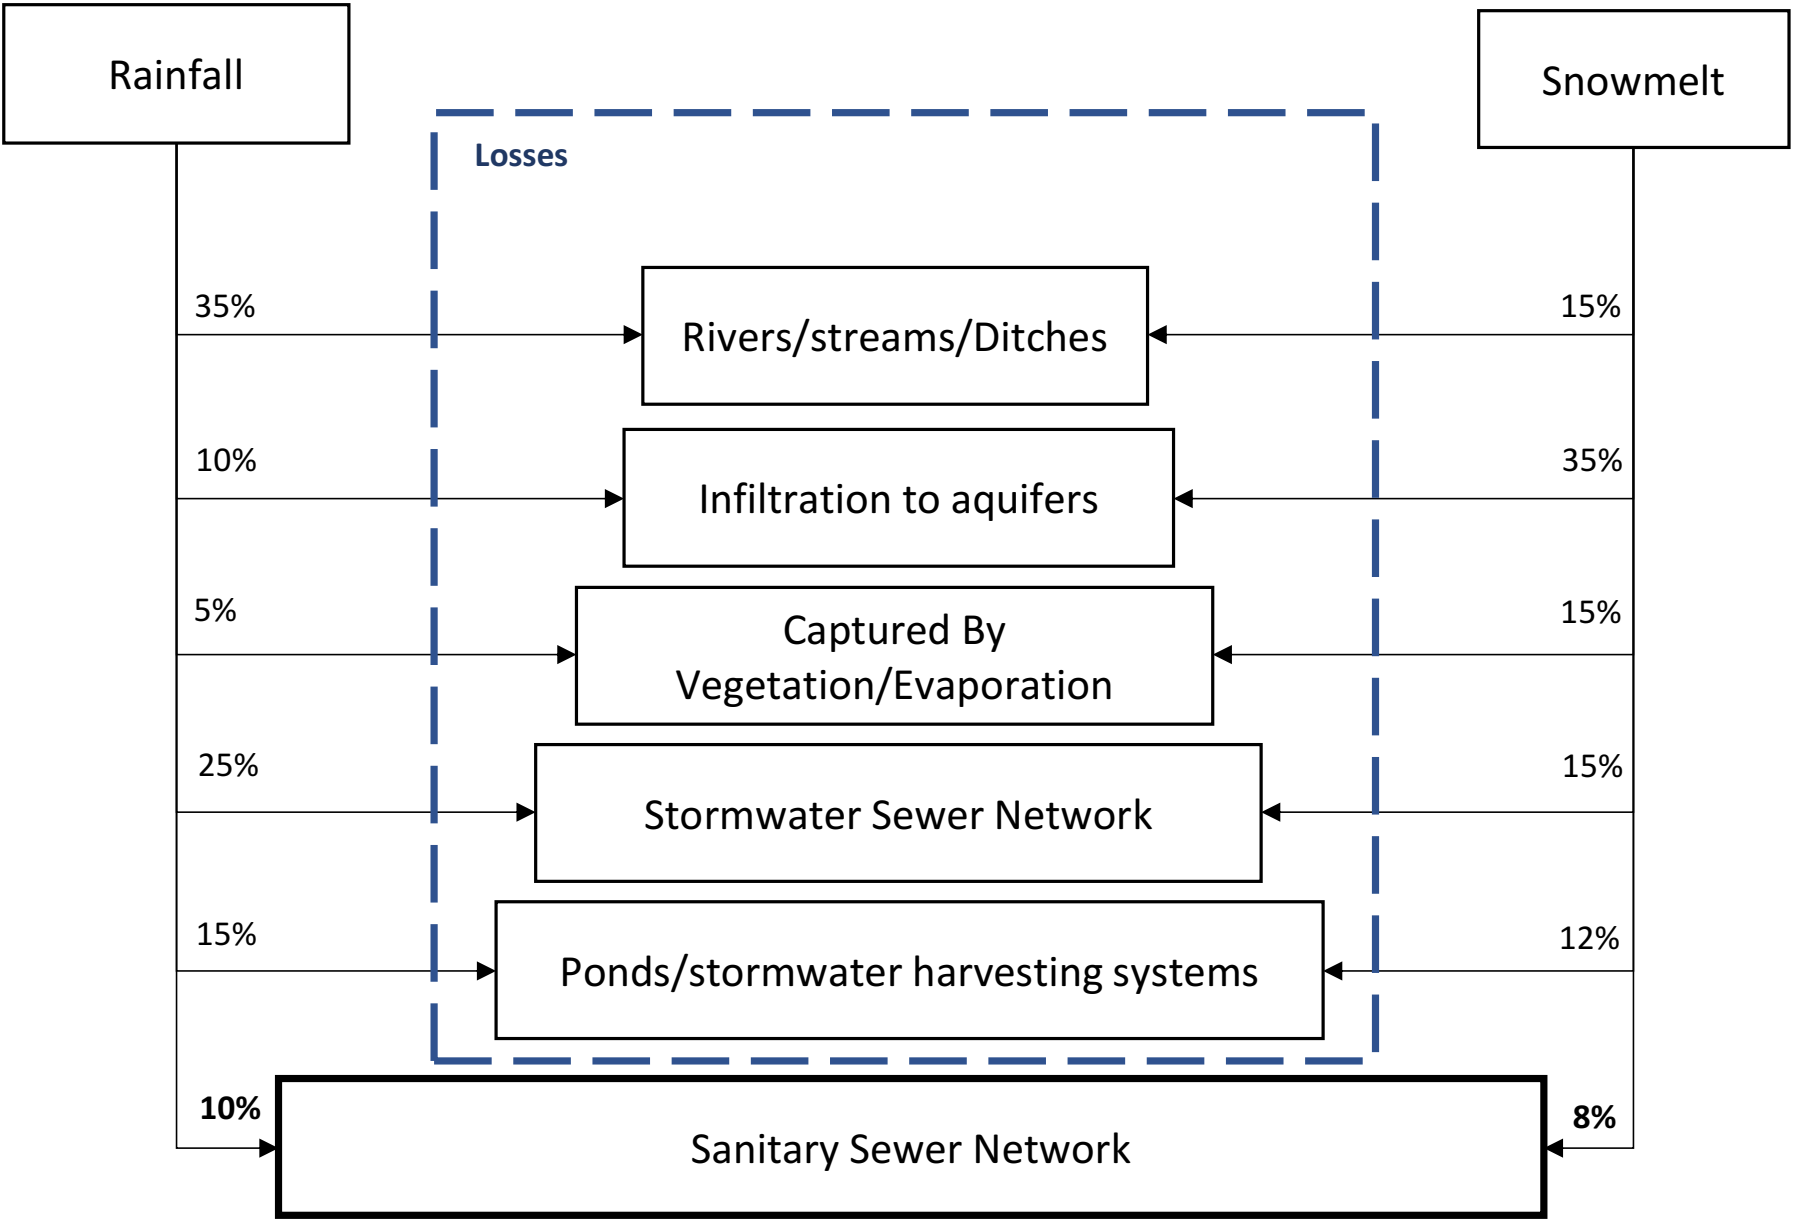
\includegraphics[scale=0.4]{figures/losses.png}
	\caption{Precipitation Losses relative to a Sanitary Sewer Network}
	\label{fig:losses}
\end{figure}

\section{Methods to Quantify Rainfall Dependent Infiltration and Inflow}


As mentioned on section 1. There are different ways stormwater or snowmelt finds its way into the sanitary sewer lines which ideally would have only wastewater from urban developments such as households, commercial centers, factories, etc.  Sanitary sewer networks’ flow increase can be trigged by an event such as a storm or elevation of the groundwater table. From rainfall or snowmelt water flows over the soil surface and inflows to the sanitary sewer through manhole leaky covers or directly from roof-drain and foundation connections. The flow increases in the sanitary sewer due to inflow is generally observed few hours after the beginning of the storm or snowmelt. As depicted in figure X, rainfall or snowmelt   Once the water infiltrates, it moves through the soil porous with a much slower velocity due to the characteristics of the groundwater flow. Infiltration of groundwater flow which reaches the elevation of pipe. Direct roof drain connections. Groundwater infiltration from saturated soil.   
There are many processes where. Function of the infiltration, groundwater flow, surface runoff, flow through pipe fissures.

Rainfall dependent infiltration and inflow have been modeled with different methods. Bennet (1999) (Bennett et al. 1999) carried a literature review and case study of around 10 different methods for quantifying RDII. 
The study concluded that only the regression and unit hydrograph methods are suitable when applying continuous simulation for long-term modelling. The unit hydrograph (UH) method also provided the best consistent match to storm peaks. Vallabhaneni and Burguess (2007) (Vallabhaneni and Burgess 2007) and U.S. EPA (2008) (Epa et al. n.d.) also considered sewer network rehabilitation capabilities as a factor for evaluation of the methods and suggested that regression should be used when more than 2 years of recorded flow and rainfall data is available. When no flow is available, the Constant Unit Rate RDII Method seems to be useful since it accounts for spatial characteristics of the Sewershed and information of pipe characteristics and population. Moreover, U.S. EPA (2008) study concluded that Unit Hydrograph RTK method can be useful to identify if which portion of the wet-weather flow is caused by inflow and which portion is caused by infiltration. Knowing whether RDII is more impacted by inflow or infiltration is relevant when evaluating the sanitary sewer network for rehabilitation. 
It is important to mention that the studies also concluded that there is no RDII quantification method that can be universally applied, since their use depend on available data and characteristics of the catchment. The goal of Vallabhaneni and Burguess (2007) (Vallabhaneni and Burgess 2007) and U.S. EPA (2008) (Epa et al. n.d.) reviews were to choose the most suitable method to be first implemented in a toolbox named as Sanitary Sewer Overflow Analysis and Planning (SSOAP). 

%maybe include the table available in benetti or whatever for visual representation. 
%Conclude about the alternative methods described above. 

TELL HERE WHY THE CHOICE OF RDII AND SWMM

As described in section X. Two main reasons was to model snowmelt was the primary motivation to use SWMM modules and subcatchments in this study. and a model that could simulate the watershed behaviour throuout all the seasons of the year. 

%Tell that physically based model could also be achieved with other tools (mention the studies for snowmelt and groundwater)
snow = \citet{muthanna2015}
Groundwater =\citet{Robinson2015}, \citet{Moore2017}

%=======================================================================
% SWMM MODULES
%=======================================================================

\section{Physically-Based: SWMM Modules}

The use of SWMM packages in this study aimed to model four processes happening simultaneously in the watershed to simulate fast, medium and long term response observed in \ac{SSN} wet-weather flows. The four processes/SWMM modules are described here as: 1. Runoff; 2. Snowpack \& Snowmelt; 3. Infiltration; 4. Groundwater. A summary of the four modules is presented on the following sections based on \citet{Rossman2016}. 

%=======================================================================
% RAINFALL-RUNOFF
%=======================================================================

\subsection{Rainfall-Runoff} 

The area in SWMM is discretized by subcatchments. The size of each subcatchment is dependent on the purpose of the model. See section \ref{} for further discussion on subcatchment delineation for this study.
The rainfall-runoff is computed in SWMM for each one of the subcatchments using a nonlinear reservoir model as depicted in figure \ref{fig:runoffreservoir} and expressed in \ref{eqn:reservoircontinuity} \cite{Rossman2016}. 

\begin{figure}[ht]
    \centering
	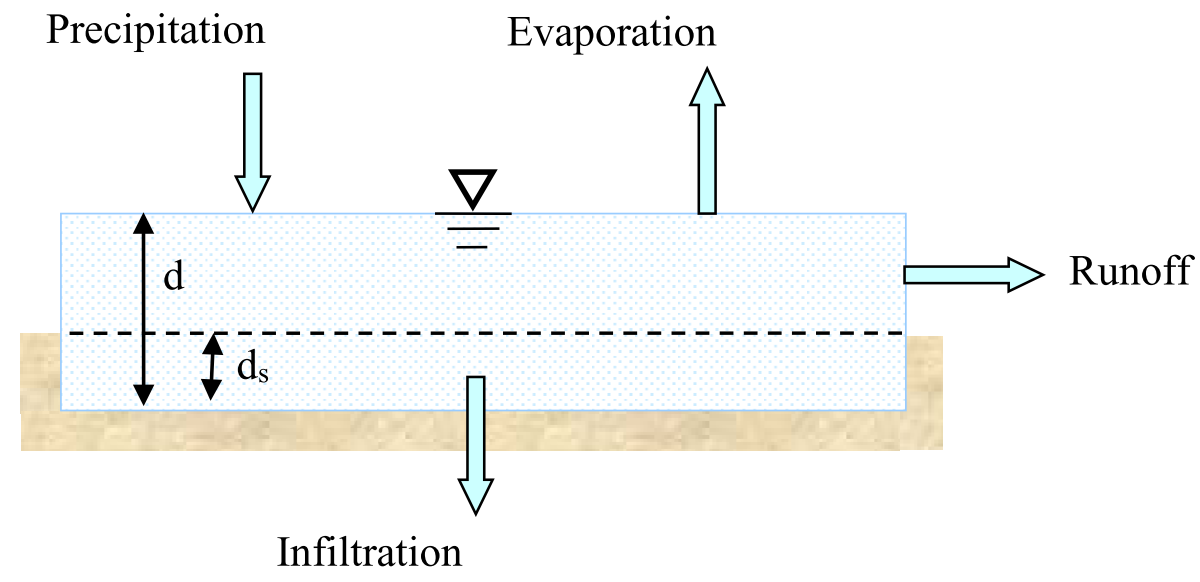
\includegraphics[scale=0.4]{figures/runoffreservoir.png}
	\caption{Nonlinear reservoir model \cite{Rossman2016}}
	\label{fig:runoffreservoir}
\end{figure}

\begin{equation}
\label{eqn:reservoircontinuity}
\frac{\partial d}{\partial t} = i - e - f - q
\end{equation}

Where:\\
i = precipitation rate [m/s]\\
e = surface evaporation rate [m/s]\\
f = infiltration rate [m/s]\\
q = runoff rate [m/s]\\

Runoff happens when water exceeds the depression storage ($D_s$) and the overland flow is assumed as uniform in a rectangular channel expressed by Gauckler–Manning–Strickler formula (\ref{eqn:manningeqn}). Each subcatchment in SWMM can be divided in three portions: 1. Pervious; 2. Impervious; 3. Impervious without $D_s$.

\begin{equation}
\label{eqn:manningeqn}
q =  \frac{1.49 \cdot W \cdot S^{1/2}}{A \cdot n} \cdot (d - d_s)^{5/3} 
\end{equation}
Where: \\
A = area [m²]\\
W = Flow width [m]\\
S = Slope [1]\\
n = Manning's roughness coefficient [s/m\textsuperscript{1/3}] \\

Runoff can be divided and routed to three different areas: 1. Outlet (node within the pipe network); 2. Pervious or impervious portion of the subcatchment; 3. Other subcatchment. The modeller can input a percent of runoff routed ($\%_{routed}$) as a parameter for SWMM model.

No information of \acf{SWSN} was assessed in this study. Therefore, the amout of stormwater that finds its way into the \ac{SWSN} is treated as a loss (see figure \ref{fig:losses}). It was also assumed that the fast response on sanitary sewer wet-weather hydrograph follows the same pattern as surface runoff. However, with a reduction in its volume. One can imagine that the hydrograph coming from a subcatchment entering the \ac{SWSN} will have the same shape as the "short term hydrograph" entering the \acf{SSN}, but with greater volume. 

The volume of water from precipitation lost to the \ac{SWSN} can be represented by two existent parameters in SWMM model: 1. depression storage ($D_s$); and/or 2. percent routed ($\%_{routed}$). Therefore, the values chosen for these two parameters in this study may differ greatly from other SWMM models focused more on modeling \ac{SWSN}. Figure \ref{fig:runoffreservoirmod} represents the conceptual difference considered in this study in comparison with the original nonlinear reservoir model.


\begin{figure}[ht]
    \centering
	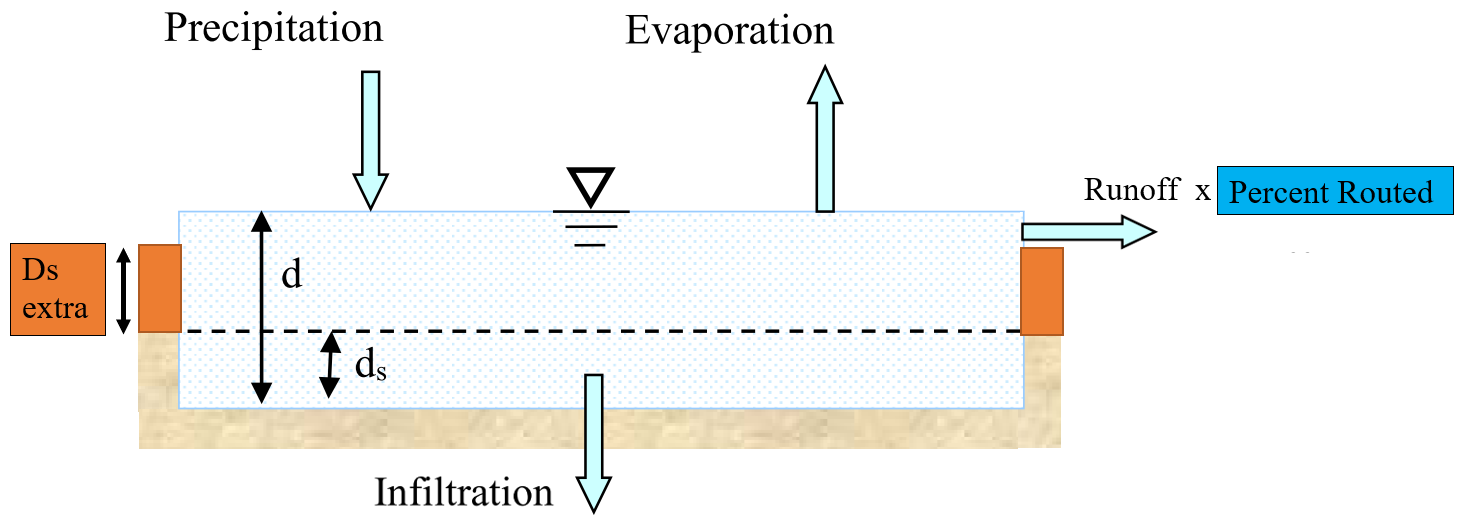
\includegraphics[scale=0.5]{figures/runoffreservoirmod.png}
	\caption{Extra $D_s$ and $\%_{routed}$ for Nonlinear reservoir model. Modified from \citet{Rossman2016}}
	\label{fig:runoffreservoirmod}
\end{figure}

$D_s$ accounts for the amount of water "absorbed" by the watershed from precipitation before runoff occurs. Wetting and ponding of the surface, and interception are usually the losses modeled by this parameter. The $D_s Extra$ and $\%_{routed}$ represented in figure \ref{fig:runoffreservoirmod} are the increment value for $D_s$ and $\%_{routed}$  to represent losses to \ac{SWSN} system. The parameter estimation is discussed later in section \ref{runoffcs}.
%=======================================================================
% SNOWPACK AND SNOWMELT
%=======================================================================

\subsection{Snowpack \& Snowmelt} \label{snowlit}

Snowpack \& snowmelt module was used to simulate the variations of flows in the \acf{SSN} occurring during winter conditions since a considerable incremental quantity of infiltration occurs during snowmelt periods as showed on the available data of section \ref{flowdata}.

Snowpack \& snowmelt calculation routines available in SWMM were based on models developed by \acf{NWS} \cite{anderson1973,anderson2006}. SWMM models the depth of water equivalent as the snowpack. The depth is increased during snow accumulation periods and decreased when snowmelt occurs. The amount of water released from the snowpack during snowmelt is transformed in precipitation rate [mm/h] and summed to the rainfall as "net precipitation" that is used as input to compute surface runoff. Therefore, snowmelt calculations are part of runoff module \cite{Rossman2016}.

Three of the key parameters for snowmelt routine are:
\begin{enumerate}
    \item $T_a$: air temperature of the current time step [C°]
    \item $T_{base}$: The base temperature of which snowmelt starts to occur [C°]
    \item $DHM$: melt coefficient [mm/h/C°]
\end{enumerate}

These three parameters are used in the linear type equation \ref{eqn:smeltdry} to compute the snowmelt [mm/h] during dry periods. Calculations of snowmelt during wet periods (greater than 0.51 mm/h) take also in consideration the wind speed and local atmospheric pressure. Refer to \citet{anderson1973,anderson2006} or \citet{Rossman2016} for detailed description of snowmelt calculations during rainfall.

\begin{equation}
\label{eqn:smeltdry}
SMELT = DHM \cdot (T_a - T_{base}) 
\end{equation}

Melt coefficient ($DHM$) varies seasonally and is calculated based on a sinusoidal equation and two user-supplied constants: 1. Minimum melt coefficient ($DHM_{min}$) which happens on December 21\textsuperscript{th}; 2. Maximum melt ($DHM_{max}$) happening on June 21\textsuperscript{th} as depicted in figure \ref{fig:meltcoeff}. 

\begin{figure}[h]
    \centering
	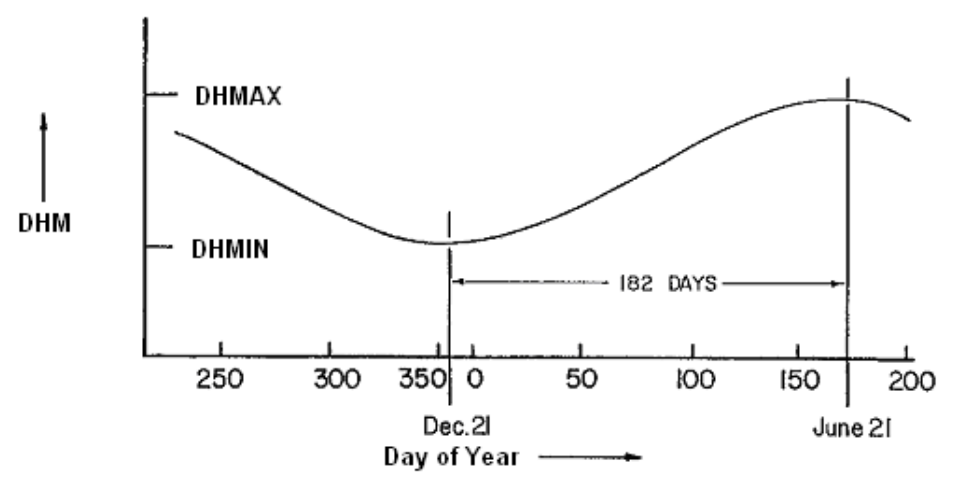
\includegraphics[scale=0.55]{figures/snowmelt_DHM.png}
	\caption{Seasonal variation of melt coefficients \cite{Rossman2016}}
	\label{fig:meltcoeff}
\end{figure}

 Before snowmelt occurs, the snowpack status has to be assessed. For this, there are two condition:
 \begin{enumerate}
    \item The snowpack has to be heated with air temperatures higher than $T_{base}$.
    \item Snowmelt has to fill the voids within the snowpack. Meaning that there is a quantity of water contained in the snowpack and it is considered to be a fraction of the "depth of water equivalent" and named as fraction of free water capacity ($FWC$). 
\end{enumerate}
  
The heat content in the pack is calculated and $FWC$ a user-supplied value. Therefore, liquid melt will only become a component of "net precipitation" after the two conditions, above mentioned, are satisfied.

 The difference between heat content of the snowpack and $T_{base}$ is named as "cold content" ($COLDC$). This variable is used to compute how much heat is necessary to be transfered to the snowpack before snowmelt can occur, as the first condition metioned above. The $COLDC$ value is updated every time step based on the heat transfer between the pack and the atmosphere. The variation of the cold content ($\Delta CC$) is calculated every time step assuming a negative value during melting periods. The following two user-supplied constant fractions are necessary to compute $\Delta CC$:
\begin{enumerate}
    \item $RNM$: Negative melt ratio [fraction]
    \item $TIPM$: ATI weight ratio [fraction]
\end{enumerate}

The rate of which heat transfer occurs is calculated based on SWMM's internal parameter of antecedent temperature index ($ATI$) which is function of $T_a$ and $TIPM$. Values of $TIPM$ towards tending to zero represent a thicker pack which warms and cools slowly as a greater weight is given to more antecedent temperatures. Equation \ref{eqn:ddcdry} is used when $T_a$ < $T_{base}$ and equation \ref{eqn:ddcwet} when $T_a$ > $T_{base}$ \cite{Rossman2016}. 

\begin{equation}
\label{eqn:ddcdry}
\Delta CC = RNM \cdot DHM \cdot (ATI - T_a) \cdot Time Step
\end{equation}

\begin{equation}
\label{eqn:ddcwet}
\Delta CC = - SNOWMELT \cdot RNM \cdot Time Step
\end{equation}

The Negative Melt Ratio ($RNM$) in equations \ref{eqn:ddcdry} and \ref{eqn:ddcwet} is used to account for a reduced heat transfer during periods without "actual liquid melt".
Snow plowing and areal depletion were not used in this study for lack of data and simplicity.
Other three parameters used were:

\begin{enumerate}
    \item $U$: Monthly average wind speed [m/s]
    \item $Z_{el}$: elevation above mean sea level [m]
    \item $SNOTMP$: Dividing temperature between snowfall and rainfall [C°]
    \item $SCF$: Snow catch factor [ratio]
\end{enumerate}

Where 1. and 2. were used to compute the influence of wind speed on the melting of snow during rainfall periods and 3. and 4. used to define the amount of snowfall from raw precipitation input data.


%Snow plowing routine was not utilized in this study for three reasons: 1. No data of snow plowing routines were assessed for the study area; 2. Assumption of no transport of snow among subcatchments; 3. Plowing of snow from impervious to pervious areas within the subcatchment assumed to be negligible since snowmelt can be routed to the pervious areas within SWMM's runoff module.

Table \ref{tbl:snowparam} depict all parameters used for the snowpack \& snowmelt module in this study and their proposed range based on other study cases available in the literature. 


\begin{table}[h]
\caption{Snowpack \& Snowmelt parameters range\cite{Rossman2016}}
\label{tbl:snowparam}
\centering
\begin{tabular}{lcc}
\toprule
\textbf{Parameter}                                                                                                           & \textbf{Proposed Range}                      & \textbf{Units}                     \\ \hline
SNOTMP                                                                                                                       & 0 - 2                                        & {[}°C{]}                           \\
SCF                                                                                                                          & 1 - 2                                     & {[}1{]}                            \\
T\textsubscript{base}                                                                                       & -4 - 0                                       & {[}°C{]}                           \\
\begin{tabular}[c]{@{}l@{}}DHM\textsubscript{min - max} \end{tabular} & 0.019 - 0.11                                 & {[}mm/°C-h{]}                      \\
RNM                                                                                                                          & 0 - 1                                        & {[}1{]}                            \\
FWFRAC                                                                                                                       & 0.01 - 0.25                                   & {[}1{]}                            \\
TIPM                                                                                                                         & 0 - 1                                        & {[}1{]}                            \\
T\textsubscript{a}; Z\textsubscript{el}; $U$                                               & \multicolumn{2}{c}{Location Based (see section \ref{meteodata})}
\end{tabular}
\end{table}

RNM and TIPM bare the full possible range. However, suggestions available in the literature were used as initial values in this study. All other ranges of parameters in \ref{tbl:snowparam}, exept by $DHM_{min - max}$, were proposed as suggested by \citeauthor{Rossman2016} \citeyearpar{Rossman2016} in the SWMM hydrology reference manual \cite{Rossman2016}.

\citeauthor{Tikkanen2013} \citeyearpar{Tikkanen2013} suggested values for the degree-hour melt coefficients ($DHM_{min - max}$) when modelling a catchment in Finland based on values calibrated by \citeauthor{valeo2004} \citeyearpar{valeo2004} for a catchment in Calgari, Canada. \citeauthor{Tikkanen2013} used reduced values in comparison to \citeauthor{valeo2004} to account for fewer solar radiation due to difference in latitude. \citeauthor{valeo2004} calibrated different values of $DHM_{min - max}$ for snow covered pervious and impervious areas varying from 0.02 for $DHM_{min}$ to 0.150 $DHM_{max}$. Therefore, the proposed range in this study was based on \citeauthor{Tikkanen2013} and \citeauthor{valeo2004} findings.

%=======================================================================
% INFILTRATION
%=======================================================================

\subsection{Infiltration} \label{infiltration}

An infiltration model was used in this study to assess long-term simulations (up to 6 months) of the winter periods using snowmelt routine. As \acf{GWI} is one of the components of \acf{SSN} flows, an aquifer and groundwater inflow models were included. The gradient of groundwater infiltration to the \ac{SSN} is dependent on the water table elevation (see section \ref{groundwater}). Therefore, the infiltration routine was included as a way to recharge the modeled aquifer varying the saturated zone elevation (water table) providing a connection between effective precipitation and the \ac{GWI} component.

SWMM version 5.1 package offers the modeller five different infiltration models. The Modified Horton method \cite{akan1992,akan2003} was chosen among the options for three main reasons: 1. it is simply one of the default methods available in SWMM;  2. it has the same parameters as the well-known Horton method which parameter estimates are suggested in \citet{Rossman2016}; 3. Appears to be more accurate low intensity rainfall events than the original Horton method \cite{Rossman2016}. 

The two governing equations of the method describes the infiltration capacity decay during wet periods \ref{eqn:mhortondecay} and its recovery curve during dry periods \ref{eqn:mhortonrecoveryintegrated} and an example of these two curves and how the infiltration capacity would change over time is plotted in figure \ref{fig:horton}. 

\begin{figure}[h]
    \centering
	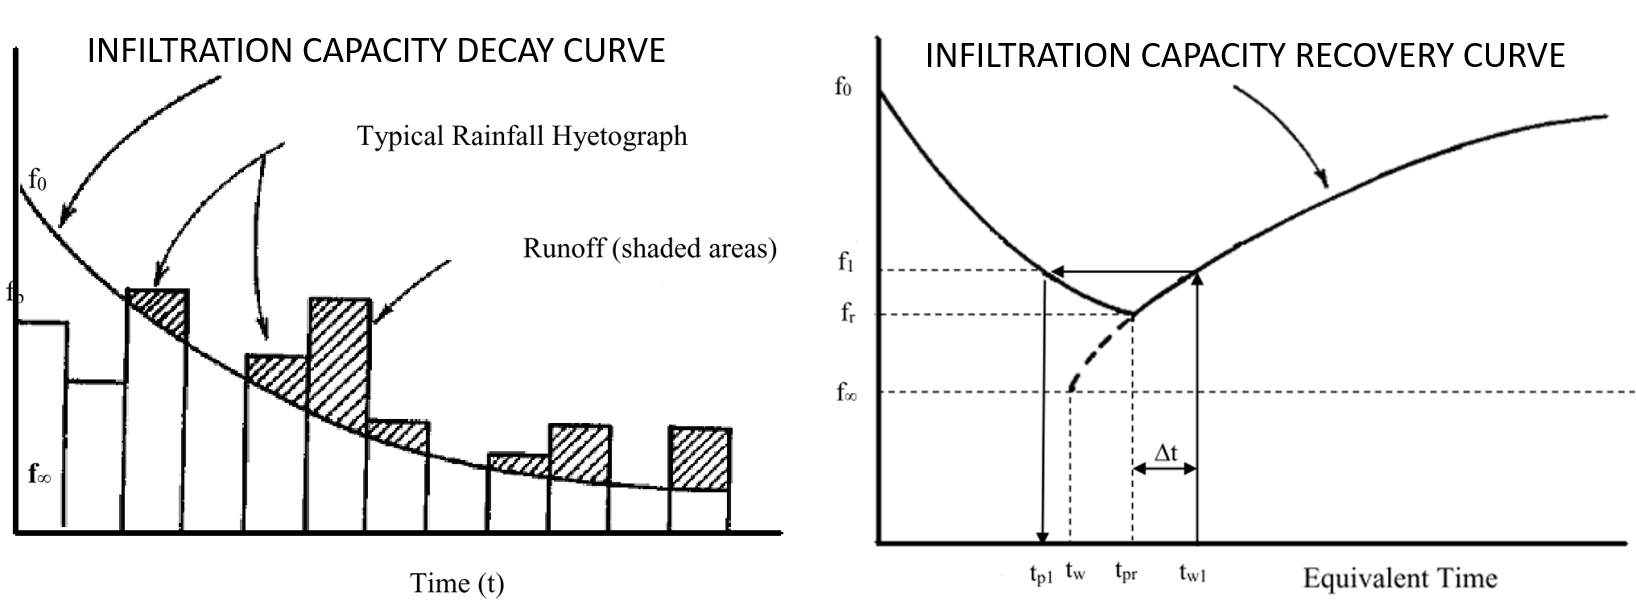
\includegraphics[scale=0.45]{figures/hortoncurves.png}
	\caption{Horton infiltration capacity decay and recovery curves. Modified from \cite{Rossman2016}}
	\label{fig:horton}
\end{figure}

\begin{equation}
\label{eqn:mhortondecay}
F = f_\infty \cdot t + \frac{(f_0 - f_\infty)}{k_d} \cdot (1 - e^{-k_d\cdot t})
\end{equation}
Where: \\
\indent $F$ = cumulative infiltration capacity [ft] \\
\indent $f_\infty$ = minimum or equilibrium value of infiltration capacity at $t = \infty$  [ft/sec] \\
\indent $f_0$ = maximum or initial value of infiltration capacity at $t = 0$ [ft/sec] \\
\indent $t$ = equivalent time [sec] \\
\indent $k_d$ = decay coefficient [sec\textsuperscript{-1}] \\

It is worth to mention that \ref{eqn:mhortondecay} is an integrated form of Horton's original equation. SWMM uses integrated form to consider the intensity of the rainfall event also as a function of the infiltration capacity reduction \cite{Rossman2016}. 


\begin{equation}
\label{eqn:mhortonrecovery}
\frac{df_r}{dt} = kr \cdot (f_0 - f_r) 
\end{equation}
Where: \\

\indent $f_r$ = infiltration capacity during recovery [ft] \\
\indent $f_{r0}$ = maximum or initial value of infiltration capacity at $t = 0$ [ft/sec] \\
\indent $k_r$ = regeneration coefficient [1/sec] \\
\indent $t$ = time [sec] \\

the infiltration capacity at time $t$ after integrating \ref{eqn:mhortonrecovery} when infiltration capacity is $f_{r0}$ is:

\begin{equation}
\label{eqn:mhortonrecoveryintegrated}
f_r =  f_0 - (f_0 - f_{r0}) \cdot e^{-k_d \cdot t}
\end{equation}
    
SWMM computation scheme first checks for wet-period (rainfall/snowmelt) or dry period to apply either of the equations \ref{eqn:mhortondecay} or \ref{eqn:mhortonrecoveryintegrated}  and compute the current infiltration capacity and the amount of water infiltrating the soil. More details of the equations and computational scheme are available in \citet{Rossman2016}.

Table \ref{tbl:infparam} presents a rough estimate of the range of four input parameters for Horton infiltration model. The range was extracted from EPA SWMM user help. 
 

\begin{table}[h]
\caption{Modified Horton infiltration parameters range\cite{Rossman2016}}
\label{tbl:infparam}
\centering
\begin{tabular}{@{}lcll@{}}
\toprule
\textbf{Parameter}        & \multicolumn{2}{c}{\textbf{Typical Range}} & \textbf{Units}        \\ \midrule
Maximum infiltration rate & \multicolumn{2}{c}{8.5 - 254}              & mm/h                  \\
Minimum infiltration rate & \multicolumn{2}{c}{0.254 - 120.4}          & mm/h                  \\
Decay coefficient         & \multicolumn{2}{c}{2 - 7}                  & h\textsuperscript{-1}\\
Drying Time               & \multicolumn{2}{c}{2 - 14}                 & days                  \\ \bottomrule
\end{tabular}
\end{table}


%=======================================================================
% AQUIFER AND GROUNDWATER
%=======================================================================

\subsection{Aquifer \& Groundwater Flow} \label{groundwater}
 
There are medium and long term wet-weather infiltration observed in \acf{SSN} measured flow data. This infiltration raises the flow above its average for days or even weeks as discussed in the previous sections. It is challenging or not possible to model the short, medium and long term hydrographs using only SWMM's runoff module since its parameters such as roughness and slope would be distorted as an attempt to reproduce the delayed flows. Moreover, a short term response can occur at the same period as the medium and long term. One can imagine a high intensity rainfall happening right after a snowmelt period. A delayed portion of snowmelt infiltrates and slowly recharges the aquifer and discharges into the \ac{SSN} while rainfall causes runoff being fully discharged in minutes or hours. The Aquifer \& Groundwater Flow module of SWMM was implemented together with the aforementioned modules as an attempt to represent the most important hydrological processes happening in the sewershed. 
Aquifer in SWMM is represented as a two zones model containing an unsaturated and a saturated zone as depicted in figure \ref{fig:gwtwozoneslit}. 

\begin{figure}[h]
    \centering
	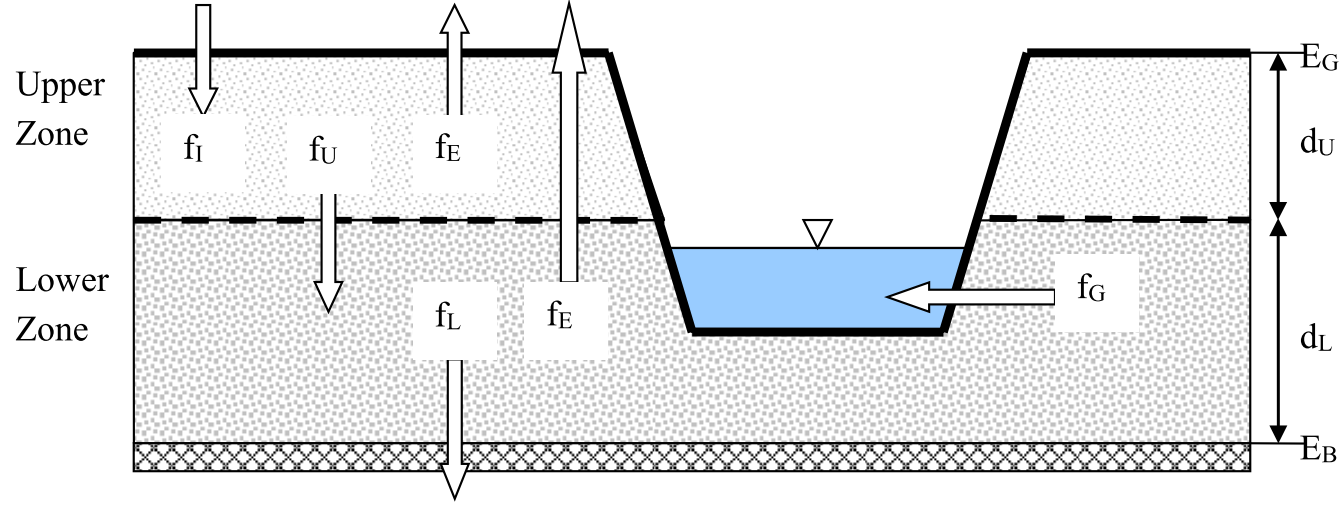
\includegraphics[scale=0.45]{figures/gwtwozoneslit.png}
	\caption{Representation of two-zone groundwater model in SWMM \cite{Rossman2016}}
	\label{fig:gwtwozoneslit}
\end{figure}

The first zone is intermediary located between the soil surface and the groundwater table. Six fluxes among soil surface and the two aquifer zones can be computed every time step varying the elevation of the groundwater table and, therefore, changing the size of the aquifer zones. The variation of the saturated zone elevation ($d_L$) affects the flow from the aquifer to the receiving node in the pipe network system ($f_G$). 

Modellers can use a customized equation to describe $f_G$ flux using available parameters from the two-zone model. SWMM's hydrology reference manual \cite{Rossman2016} mentions options such as Linear Reservoir, Dupuit-Forcheimer Lateral Seepage, and Hooghoudt's Tile Drainage. However, it is important to remember that groundwater table elevation is constant along the subcatchment limiting the representation of the pressure gradient between the saturated zone and the receiving node to the difference between $d_L$ and the elevation of water surface in the receiving node. Note that these two elevations can vary every time step and govern changes in $f_G$.


\section{Synthetic Unit Hydrograph: RTK}







\chapter{Hydraulic Model}


Write also about the Junctions invert elevations (min, max, average, histogram with number of junctions/conduits with certain invert elevation range, statistics of the network)

Picture of network

\chapter{Case Study}

\chapter{Case Study}

\section{Jokela Town}

\section{Data}

    \subsection{Sanitary Sewer Inflow}
    
    \subsection{Precipitation}
    
    \subsection{Topographic Data}
    DEM
    LAND USE
    URBAN AREA
    IMPERVIOUSNESS
    SOIL TYPE
    
    \subsection{Groundwater}

As mentioned in the literature ((Bennett et al. 1999; Vallabhaneni and Burgess 2007), (Barden et al. 2011), and others), infiltration into the sewer lines can be caused by the seasonal elevation of groundwater table or other condition that increased soil moisture content causing a temporary saturated zone. Elevation of the groundwater table around Jokela town was assessed in this section as an attempt to identify a possible correlation with seasonal variations of the water table and the flow measurements of the town’s sanitary sewer network. 
Information of water table levels was provided by the Finnish Environmental Institute (SYKE) through its open data service (“Finnish Environment Institute (SYKE) Open Environmental Information Systems” n.d.). Data of three observation wells were available surrounding Jokela town as depicted in Figure 4. The recording period and routines among the three stations varies considerably - from one record per month to one record per year.

Picture

Measurements from 2004 to 2016 from station 0118651 -located southeast from Jokela- were combined and plotted in Figure 5. Years with less than six months recorded were left out: 2007; 2008; and 2017. All the eleven years records showed an elevation on the groundwater table from March to May. 

Picture

Only yearly measurements were available for the closest station 0154356 located around 5km west from Jokela. The records are from different months, mostly during spring and summer. Therefore, assessment of monthly variation for the same year was not possible. However, the available data suggests slightly higher water table levels on average from January to June for the period of 1999-2017.

Picture

The closest observation well with data available from 2018 was 110651. Measurements from 2018 were relevant to compare with flow measurements of the same year in the sewer network. As depicted in Figure 6, the groundwater elevation period is on average from February to May. Similar pattern as observed for station 0118651. For 2018, periods of February-March and April-May were presented elevation in the groundwater table. If a similar groundwater elevation pattern also occurred for Jokela town in 2018, located 9 km away, correlation between aquifer recharge periods and higher infiltration rates into the sanitary sewer exists. 
    
    
    \subsection{Weather Forecast}

\section{Data Treatment}

\section{Jokela Sanitary Sewer Model}

    \subsection{Hydraulic Model}
    
    \subsection{Physically-Based: SWMM Modules}
        
        \subsubsection{Sewershed Delineation}
          
         \textit{GRASS - v.clean} to split where streams intersect.
         \textit{QGIS - Merge Lines} To merge streams within the same layer. 
         \textit{QGIS - Split with lines} to split the sewershed polygon where the stream crosses.
        
        
        \subsubsection{Parameter Estimation}
    
    \subsection{Synthetic Unit Hydrograph: RTK}
        
        \subsubsection{Parameter Estimation}
        
\section{Real-Time Simulations}

% \printbibliography
\bibliographystyle{plainnat}
\bibliography{library}



\end{document}
